\documentclass[a4paper,preprint]{sig-alternate}

\usepackage{times}
\usepackage{helvet}
\usepackage{courier}
\usepackage{microtype}
\usepackage{hyperref}

\frenchspacing

\toappear{}

\usepackage{blindtext}

\begin{document}

\title{Robustness \& Graph (Convolutional) Neural Networks}

\numberofauthors{1}
%
\author{
%
\alignauthor Tim Bohne\\
\email{tbohne@uni-osnabrueck.de}
}

\maketitle

\section{Introduction}

The intent of this paper is to provide a concise overview of the current state of research in the domain of graph (convolutional) neural networks
with a focus on the robustness of these models. Since they have proven to be successful in various practical applications, 
it is quite obvious that the robustness of such models is of relevance.
After presenting some motivation and background for graph neural networks (GNNs) and particularly graph convolutional networks (GCNs)
and their possible practical applications in section \ref{sec:background}, an overview of the current state of the literature is
provided in section \ref{sec:literature}. Subsequently, the core ideas, methods, and results of the first works on certifiable
robustness of GNNs are introduced in section \ref{sec:main_section}.
Finally, there is a conclusion and a brief outlook on possible future research in section \ref{sec:conclusion}.

\section{Background}
\label{sec:background}

A currently very active research area inside the field of machine learning, or more precisely deep learning, considers models to learn
from graph inputs. Those models are called graph neural networks (GNNs). Graphs are useful data structures in complex real-life
applications such as modeling physical systems, learning molecular fingerprints, controlling traffic networks, and recommending 
friends in social networks.\cite{article}
Therefore, it is reasonable to think about combining graphs as data structures with state-of-the-art machine learning models.
However, these tasks require dealing with non-Euclidean graph data that contains rich relational information between elements and
cannot be well handled by traditional deep learning models which usually work with data represented in the Euclidean domain, e.g. in the
fields of computer vision (images) or natural language processing (text).\cite{article}
There are numerous reports of convincing performance of GNNs in practical applications (e.g. \cite{NIPS2015_f9be311e},
\cite{hamilton2018inductive}, \cite{trivedi2017knowevolve}), especially in the task of semi-supervised node classification.\cite{xu2019topology}
Further typical applications for graphs as non-Euclidean data structure in machine learning are link prediction and clustering.\cite{zhou2019graph}
In summary, GNNs are models to conduct deep learning with graph data.

\subsection{Motivation}

One of the most successful types of models in the field of deep learning is the convolutional neural network (CNN).
GNNs are motivated by CNNs which are capable of extracting and composing multi-scale localized spatial features
for features of high representational power, but can only operate on Euclidean data like images and text.\cite{article}
Thus, the idea is to generalize CNNs to graphs.\newline
Another motivation comes from graph embedding, which learns to represent graph nodes, edges, or subgraphs in low-dimensional vectors.\cite{article}
Liu et al. also highlight that traditional machine learning approaches for graph analysis rely on hand-engineered features which causes them
to be rather inflexible and expensive.

\vfill
\pagebreak

\subsection{Graph Neural Networks}

In this section, the basic graph neural network model proposed by Scarselli et al. \cite{4700287} gets introduced
based on the description in \textit{'Introduction to graph neural networks'}\cite{article}.
The goal of a GNN is to learn a state embedding $h_v \in \mathbb{R}^S$ for each node that is used to produce an 
output $o_v$, e.g. the distribution of the predicted node label.
The original GNN model works with an undirected homogeneous graph where each node $v$ in the graph has its input features $x_v$
as well as a set of edges $co[v]$ and neighbors $ne[v]$. The authors illustrate the structure with the example in fig. \ref{fig:graph}
where $x_{1}$ is the input feature of $l_1$, $co[l_1]$ contains the edges $\{l_{(1, 2)}, l_{(1, 4)}, l_{(1, 6)}, l_{(3, 1)}\}$, and 
$ne[l_1]$ contains the nodes $\{l_2, l_3, l_4, l_6\}$.

\begin{figure}[h]
    \centering
    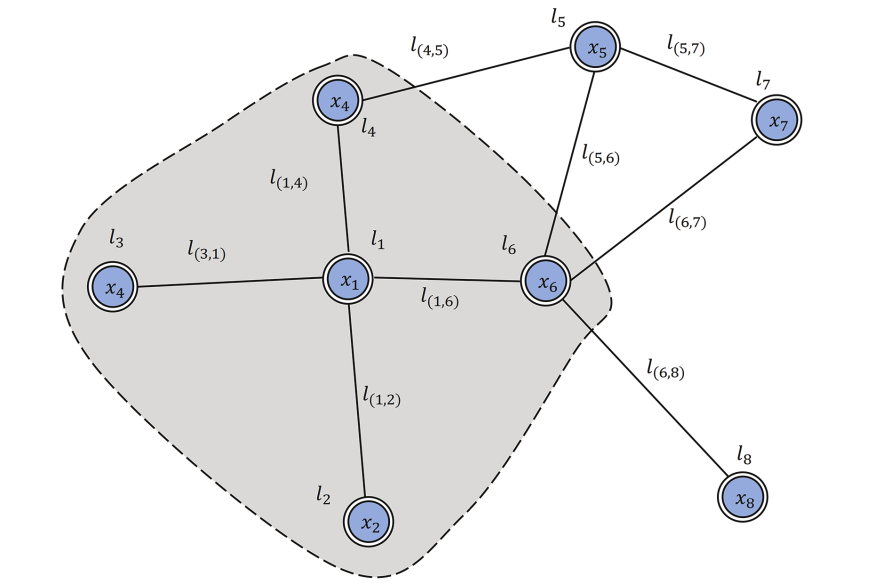
\includegraphics[width=0.4\textwidth]{img/graph.png}
    \caption{Example of the graph based on Scarselli et al. \cite{article}}
    \label{fig:graph}
\end{figure}

There are two important functions, $f$ updates the node state based on the input neighborhood and $g$ computes the output of a node.
Let $x$ be the input feature and $h$ the hidden state:
\begin{itemize}
    \item \textbf{node embedding:} $h_v = f(x_v, x_{co[v]}, h_{ne[v]}, x_{ne[v]})$
    \item \textbf{output embedding:} $o_v = g(h_v, x_v)$
\end{itemize}

Therefore, $f$ takes as input the features of the node ($x_v$), the features of its edges ($x_{co[v]}$), the states ($h_{ne[v]}$),
and the features of the nodes in its neighborhood ($x_{ne[v]}$). The node embedding $h_v$ is then used in $g$ to compute the output of $v$.
Usually, $h_v$ and $o_v$ are described in a more compact form as matrices of stacked states $H$,
outputs $O$, and features $X$ (and node features $X_N$) with $F$ and $G$ being the stacked versions of $f$ and $g$:

\begin{itemize}
    \item $H = F(H, X)$
    \item $O = G(H, X_N)$
\end{itemize}

The $(t + 1)$-th iteration of $H$ is described as $H^{t + 1} = F(H^t, X)$.
Using the target information $t_v$ for node $v$, the loss can be written as $\sum_{i=1}^p (t_i - o_i)$
where $p$ is the number of supervised nodes. The learning algorithm is based on a gradient-descent strategy.\newline

\vfill
\pagebreak

This basic GNN model provides a first step towards incorporating neural networks into the graph domain, 
but has several limitations \cite{article} which are tackled in numerous variants of GNNs such as graph convolutional networks (GCNs).\newline

\textbf{Graph Convolutional Networks}\newline

The properties that define the different variants of GNNs are typically the aggregator to gather information from each node's neighbors
and a specific updater to update the node's hidden states. \cite{zhou2019graph} In general, there is a certain functional evaluation of
a node's features together with the featuers of its neighbors (convolution). The results are then the input for the neural network.
GCN approaches are often categorized as spectral or spatial approaches. Spectral approaches
work with a spectral representation of the graph and the convolution operation is defined in the Fourier domain by 
computing the eigendecomposition of the graph Laplacian. \cite{zhou2019graph}
A simple schematic representation of a deep GCN is depicted in fig. \ref{fig:gcn}.
\begin{figure}[h]
    \centering
    \includegraphics[width=0.45\textwidth]{img/gcn.png}
    \caption{Multi-layer GCN. \cite{kipf2016semi}}
    \label{fig:gcn}
\end{figure}

\subsection{Robustness}

Besides the repeatedly demonstrated good performance, there is one big issue which is subject to a rather new branch of 
research inside the field of GNNs, which is the robustness of such models. There are several publications that analyze 
the robustness of GNNs to adversarial examples and recently there came up first approaches to strengthen
or even to certify their robustness with regard to a certain perturbation set.\newline
Recent advancements in deep neural networks for graph-structured data have led to state-of-the-art performance on recommender system benchmarks.\cite{Ying_2018}
Ying et al. describe a large-scale deep recommendation engine that they developed and deployed at a major tech company.
This example illustrates the need for robust GNNs. Although these systems may be relatively rare in practical applications, especially at
that scale, at the moment, their performance suggests that that will change soon. However, in order to be able to use such models
with a clear conscience in practical applications requires a certain degree of robustness.
The vulnerability to adversarial attacks has raised increasing concerns for applying GNNs in safety-critical applications.\cite{jin2020graph}\newline

\textbf{Adversarial Perturbations}\newline

A well-studied problem of machine learning models in general is the sensitivity to adversarial perturbations.\cite{goodfellow2015explaining}
The idea of such perturbations, which is visualized in fig. \ref{fig:adversarial_example}, is that slight changes to the input data
cause an entirely different output of the model and therefore often misclassification.

\begin{figure}[h]
    \centering
    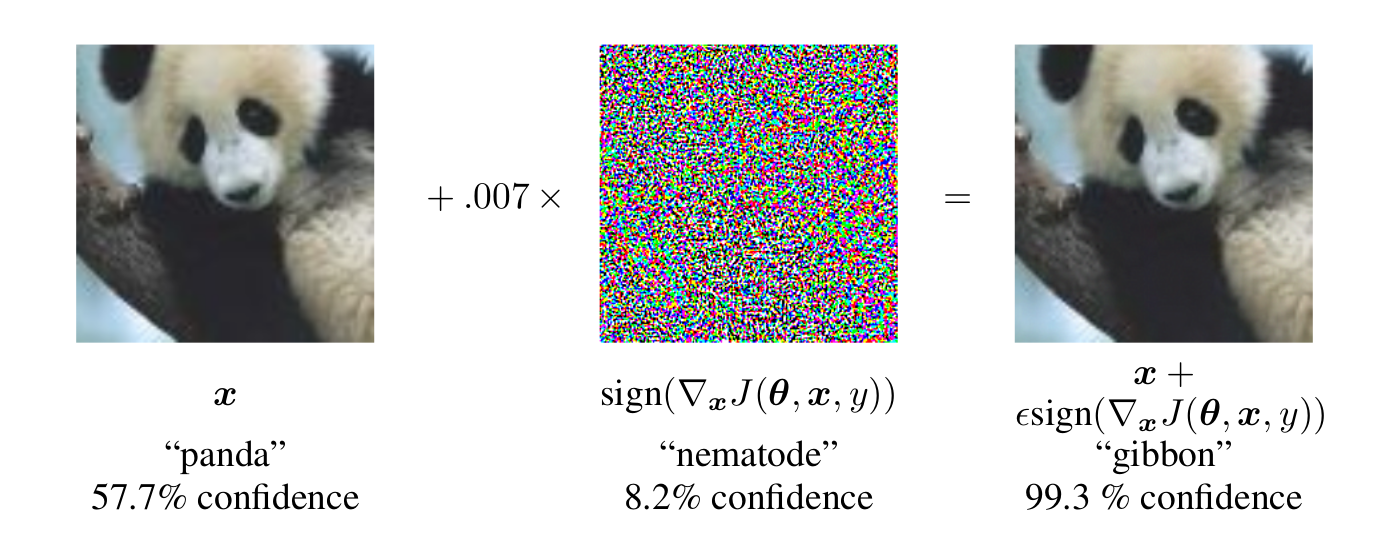
\includegraphics[width=0.5\textwidth]{img/adversarial_example.png}
    \caption{Demonstration of a fast adversarial example. \cite{goodfellow2015explaining}}
    \label{fig:adversarial_example}
\end{figure}

Goodfellow et al. \cite{goodfellow2015explaining} face that problem by adversarial training which means that they include adversarially 
perturbed examples into the training procedure to strengthen the robustness of the models. They also introduce fast methods for generating 
those adversarial examples such as displayed in fig. \ref{fig:adversarial_example}. By adding an imperceptibly small vector whose elements
are equal to the sign of the elements of the gradient of the cost function with respect to the input, they can change GoogleNet's classification
of the image.\cite{goodfellow2015explaining}\newline
Adversarial perturbations are not only a problem for classical machine learning models, but also for GNNs.
Recent works show that graph neural networks are highly non-robust with respect to adversarial attacks on both the graph
structure and the node attributes, making their outcomes unreliable.\cite{Z_gner_2019}
Similarly to the example in fig. \ref{fig:adversarial_example}, small perturbations to the graph structure and node features lead to 
misclassification of the target as depicted in fig. \ref{fig:adversarial_GNN}.

\begin{figure}[h]
    \centering
    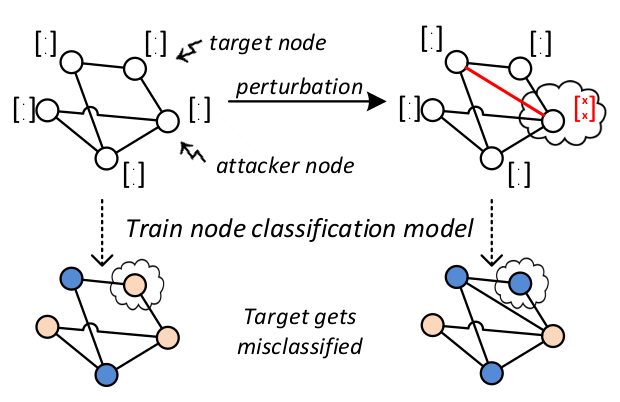
\includegraphics[width=0.35\textwidth]{img/adversarial_GNN.png}
    \caption{Small perturbations of the graph structure and node features lead to misclassification of the target. \cite{Z_gner_2018}}
    \label{fig:adversarial_GNN}
\end{figure}

\section{Literature Review}
\label{sec:literature}

This section will provide an overview of the current state of research in the domain of robust GNNs which could be divided
roughly into three important phases.
The first phase was to show that GNNs are indeed vulnerable to adversarial perturbations of the graph structure and the node attributes (cf. \ref{sec:rev1}).
Afterwards, in the second phase, several publications introduced defense mechanisms against such attacks or novel training procedures 
to strengthen the robustness of the models in some scenarios (cf. \ref{sec:rev2}). Only recently, the third phase began in which first approaches appeared
that are able to not only provide mitigations to adversarial attacks in some scenarios, but to give provable guarantees about the (non-)robustness 
of a model which is key to use them in safety-critical applications in the real world (cf. \ref{sec:rev3}). Because of the relevance of the last phase, which 
is an important step in the process of bringing the convincingly performing GNN models into the real world, the main focus of the following sections
will be on publications from that phase.

\subsection{Vulnerability of GNNs to adversarial perturbations}
\label{sec:rev1}

Dai et al. \cite{dai2018adversarial} focus on adversarial attacks on graph structured data that fool the model by modifying the
combinatorial structure of the data. They use synthetic and real-world data to show that a family of GNN models is vulnerable
to these attacks in both graph-level and node-level classification tasks.
Another approach for adversarial attacks on graph structured data is proposed by Zügner et al. \cite{Z_gner_2018} who focus on node classification
via graph convolutional networks.
The authors claim that especially in domains where GNNs are used, e.g. the web, adversaries are common and that it is therefore important
to investigate the robustness of such models. They study adversarial attacks on attributed graphs and distinguish between
adversarial attacks on the node's features and the graph structure. Their results suggest that the accuracy of node classification
significantly drops even for only a few perturbations which clearly motivates reflections on the robustness of such models, especially
when considering practical applications.
So far, adversarial attacks were introduced as a quite vague concept. Zügner et al. \cite{zuegner2019adversarial}
define them as small deliberate perturbations of data samples in order to achieve the outcome desired by the attacker
and propose three categories to be considered in the attack model. Those categories, that are discussed in detail in section \ref{},
allow more precise considerations of a model's weaknesses and robustness and are later used to compare and interpret results of 
different approaches. Furthermore, they confirm previous claims that small graph perturbations consistently lead to a strong decrease 
in performance for GCNs.

\subsection{Defense mechanisms}
\label{sec:rev2}

Since the fact that GNNs are vulnerable to adversarial perturbations was confirmed by many publications, the next natural question to ask
is how to defend them against such attacks. 
Direct extension of defense algorithms for classical neural networks based on adversarial samples meets with immediate challenge because
computing the adversarial network costs substantially. \cite{Jin2020} The authors propose to address this issue by perturbing the latent 
representations in GCNs, which not only increases efficiency because there is no need to generate adversarial networks, but also attains 
improved robustness and accuracy. They apply their framework of latent adversarial training on graphs to node classification,
link prediction, and recommender systems and are able to confirm superior robustness in experiments.
When considering the robustness of GNNs, it is of course quite important to have efficient and effective attack methods to test with.
Xu et al. \cite{xu2019topology} present a gradient-based attack method that facilitates the difficulty of tackling discrete graph data
and leads to a noticeable decrease in classification performance. Furthermore, they propose an optimization-based adversarial training
for GNNs which yields higher robustness without sacrificing classification accuracy.
Zhu et al. \cite{10.1145/3292500.3330851} propose Robust GCN (RGCN), a novel model that fortifies GCNs against adversarial attacks.
Instead of representing  nodes as vectors, they adopt Gaussian distributions as the hidden representations of nodes in each
convolutional layer which allows the model to automatically absorb the effects of adversarial changes in the variances of the Gaussian distributions.
Moreover, to remedy the propagation of adversarial attacks in GCNs, they propose a variance-based attention mechanism, i.e. assigning different
weights to node neighborhoods according to their variances when performing convolutions. Their experimental evaluation suggests that
the method can effectively improve the robustness of GCNs.\newline
Another approach to enhance the robustness of GCNs is proposed by Chen et al. \cite{Chen2020} and is based on the idea that
edge manipulations play a key role in graph adversarial attacks. They design a biased graph-sampling scheme to drop graph connections
such that random, sparse and deformed subgraphs are constructed for training which mitigates the sensitivity 
to edge manipulations, and thus enhances the robustness of the models. Their experimental results validate the effectiveness 
against adversarial attacks.
The idea, the approach of Jin et al \cite{jin2020graph} is based on, is to defend adversarial attacks by cleaning up the perturbed graph.
The authors state that real-world graphs share some intrinsic properties as they are often low-rank, sparse, and the features of two adjacent
nodes tend to be similar and that adversarial attacks are likely to violate these properties.
They introduce the framework Pro-GNN, which can jointly learn a structural graph and a robust GNN model from the perturbed graph guided by
these properties and are able to show that the framework achieves significantly better performance compared with state-of-the-art 
defense methods.
Finally, Wang et al. \cite{wang2019graphdefense} present with GraphDefense an algorithm to improve the robustness of GCNs
against adversarial attacks on graph structures. Moreover, they discuss crucial characteristics of defense methods in general to improve 
the robustness.

\subsection{Certifiable Robustness}
\label{sec:rev3}

When considering safety-critical applications, it is not only required to be able to defend the system in some scenarios, but there
have to be guarantees about the safety of the system.
Bojchevski et al. \cite{bojchevski2019certifiable} present a first method for verifying certifiable
(non-)robustness to perturbations of the graph structure for a general class of models including GNNs. Additionally, they investigate robust 
training procedures that increase the number of certifiably robust nodes while maintaining or even improving the predictive accuracy.
However, their work is limited to a specific class of graph models based on PageRank, not covering the highly important principle of graph convolutional
networks. \cite{10.1145/3394486.3403217}
Zügner et al. \cite{Z_gner_2019} propose a first method for certifiable (non-)robustness of GCNs with respect to 
perturbations of the node attributes. If a node has been certified with their method, it is guaranteed to be robust under any
possible perturbation given the attack model. Likewise, they can certify non-robustness and present a robust semi-supervised training
procedure which improves the robustness with only minimal effect on the predictive accuracy.
Recently, Zügner et al. \cite{10.1145/3394486.3403217} tackle the problem of GCNs under perturbation of the graph structure and introduce a method
for certifying their robustness. They show how the problem can be expressed as a well-studied jointly constrained bilinear program and
present a branch-and-bound algorithm to obtain lower bounds on the global optimum. The problem gets decomposed into sub-problems that can
be formulated as linear programs and therefore be solved using highly optimized LP-solvers (e.g. CPLEX).
The first certified robustness guarantee of any GNN for both node and graph classifications against structural perturbation
is provided by Wang et al.\cite{wang2020certified} Their approach is based on a recently developed technique called randomized smoothing,
which they extend to graph data.

\section{Certifiable robustness of graph neural networks}
\label{sec:main_section}

As seen in the previous sections, GNNs are highly non-robust with respect to adversarial attacks on the graph
structure and the node attributes. This section will provide an overview of the very important and only recently started 
third phase of research in the domain of robust GNNs which aims to give provable guarantees about the (non-)robustness of a model 
which is key to use them in safety-critical applications in the real world.\newline
The first work on verifying certifiable (non-)robustness to graph perturbations for a general class of models that includes GNNs and label/feature
propagation is provided by Bojchevski et al. \cite{bojchevski2019certifiable}. By exploiting connections to PageRank and Markov decision processes,
their certificates can be efficiently computed. Additionally, they investigate robust training procedures that increase the number of certifiably
robust nodes while maintaining or even improving the predictive accuracy. However, since their work is limited to a rather specific class of 
graph models based on PageRank, not covering the highly important principle of GCNs, the approach will not be further discussed in this work.\newline
After a slightly deeper consideration of the approaches of Zügner et al. providing first robustness certificates for GCNs with respect to 
perturbations of the node attributes in section \ref{sec:paper_two} and the graph structure in \ref{sec:paper_three},
a brief overview of the latest work on certifiable robustness of GNNs against adversarial structural perturbations is provided 
in section \ref{sec:paper_four}.\newline

\subsection{Robustness of GCNs with respect to perturbations of the node attributes}
\label{sec:paper_two}

In this section, the approach of Zügner et al. \cite{Z_gner_2019} will be described
in which the authors propose a first method for provable (non-)robustness of graph convolutional networks with respect
to perturbations of the node attributes.\newline
They consider the case of binary node attributes and perturbations that are $L_0$-bounded. If a node has been certified
with their method, it is guaranteed to be robust under any possible perturbation given the attack model. Likewise, they can
certify non-robustness. The proposed semi-supervised training procedure that treats labeled and unlabeled nodes jointly,
significantly improves the robustness of the GNN with only minimal effect on the predictive accuracy.
As a core challenge, the authors identify that in a GNN, a node's prediction is also effected when perturbing other nodes in the graph
which makes the space of possible perturbations large. The main question of the work is:
\begin{quote}
How to make sure that small changes to the input data do not have a dramatic effect to a GNN?
\end{quote}

\textbf{Certificates}\newline

Given a trained GNN, the authors can give robustness certificates that state that a
node is robust with regard to a certain space of perturbations. If the certificate
holds, it is guaranteed that no perturbation in the considered space exists
which will change the node's prediction. Furthermore, they provide non-robustness
certificates realized by providing adversarial examples.\newline

\textbf{Robust Training}\newline

Besides the certification technique, a learning principle which improves the robustness of a GNN
by making it less sensitive to perturbations while still ensuring high accuracy for node classification, is proposed.\newline

\textbf{Difference to existing work on provable robustness}\newline

The authors describe the main difference in the fact that existing work on provable robustness for classical neural networks
does not consider graphs with their relational dependencies which lead to perturbations of multiple instances simultaneously.
For this, they introduce a novel space of perturbations where the perturbation budget is constrained locally and globally.
The key idea that they exploit is that they estimate the worst-case change in the predictions obtained by the GNN under
the space of perturbations. If the worst possible change is small, the GNN is robust. Since the worst-case cannot be computed
efficiently, they provide bounds on the value and derive relaxations of the GNN and the perturbation space, 
enabling efficient computation. Finally, they show on various graph datasets that GNNs trained in the traditional way are not robust. 
Using their robust training, they can dramatically improve the robustness and therefore improve the reliability of GNNs.

\subsubsection{Certifying the robustness of a given GNN}

The first goal is to derive an efficient principle for robustness certificates. Given a trained GNN and a specific node $t$ under consideration,
their goal is to provide a certificate which guarantees that the prediction made for $t$ will not change even if the data gets perturbed.
If the certificate is provided, the prediction for this node is robust under any admissible perturbation.\newline
In a GNN with $L$ layers, the output of node $t$ only depends on the nodes in its $L-1$ hop neighborhood
which allows them to reduce the entries that are required to compute the output for the target node $t$. That drastically improves the scalability
by reducing the size of the neural network and potential perturbations. Given that sliced version of the GNN, they define their actual
task which is to verify whether no admissible perturbation changes the prediction of the target node $t$.\newline

Given a graph $G = (A, X)$, a target node $t$, and a GNN with parameters $\theta$. $A$ is the adjacency matrix and $X$ represents the nodes' features.
The sliced versions of $A$ and $X$ are denoted as $\dot{A}$ and $\dot{X}$. $y^*$ denotes the class of node $t$ given by ground truth or predicted.
One important aspect, the authors emphasize, is that it is crucial to obtain certificates that reflect realistic attacks.
They define the set of admissible perturbations by limiting the number of changes to the original attributes with a perturbation
budget $Q \in \mathbb{N}$ and measure the $L_0$ norm in the change to $\dot{X}$. Since in a graph setting, an adversary can attack the target node
by also changing the node attributes of its $L-1$ hop neighborhood, $Q$ acts as global perturbation budget. The perturbations are also limited locally
by a budget of $q$. The worst case margin $m^t$ between the classes $y^*$ and $y$ for a node $t$ achievable under some set
of admissible perturbations to the model attributes is given by
\begin{gather} 
\label{eq:1}
    m^t (y^*, y) := \min_{\tilde{X}} f_{\theta}^t(\tilde{X}, \dot{A})_{y^*} - f_{\theta}^t(\tilde{X}, \dot{A})_y \\
    s.t. \quad \tilde{X} \in X_{q, Q} (\dot{X})
\end{gather}
where $f_{\theta}^t(\dot{X}, \dot{A})$ represents the output of the sliced GNN and $X_{q, Q} (\dot{X})$ is the set
of admissible perturbations to the node attributes.
If $m^t (y^*, y) > 0$ for all $y \neq y^*$, the GNN is certifiably robust with regard to node $t$ and $X_{q, Q}$. 
Thus, if the minimum is positive, there exists no adversarial example within the admissible perturbations that leads 
to the classifier changing its prediction to the other class.\newline

The authors identify two major obstacles in efficiently finding the minimum in \ref{eq:1}.
First, the data domain is discrete which makes optimization often intractable. Second, the GNN ($f_{\theta}^t$) is nonconvex
due to the nonlinear activation function in the neural network. They tackle those issues by efficiently computing lower bounds
on the minimum of the original problem by performing relaxations of the neural network and the data domain.
If a lower bound is positive, the classifier is robust w.r.t. the set of admissible perturbations.
To make the objective function convex, they have to find a convex relaxation of the ReLU activation function. There are many ways to achieve this
in the literature and the authors follow one that leads to a linear objective function which is a lower bound on the minimum of the original problem.
However, directly solving it is still intractable due to the discrete data domain.

The problem is now transformed into a linear problem since besides the linear objective function, all constraints are linear as well.
While it is possible to solve LPs efficiently using highly optimized LP-solvers, the potentially large number of variables in a GNN
makes this approach rather slow. Alternatively, they consider the dual of the LP. Any dual-feasible solution 
is a lower bound on the minimum of the primal problem. If they find any dual-feasible solution for which the objective function of the dual is positive,
they know that the minimum of the primal problem has to be positive as well, guaranteeing robustness of the GNN w.r.t. any perturbation in the set.
The dual problem's specific form makes it amendable for easy optimization. Since it's not required to solve the dual problem optimally, 
any dual-feasible solution leads to a lower bound on the original problem, the computation of robustness certificates is extremely fast.
In summary, by considering the dual program, they obtain robustness certificates if the obtained (dual) values are positive for every $y \neq y^*$.
In contrast, by constructing the primal feasible perturbation, they obtain non-robustness certificates if the obtained (exact, primal) values
are negative for one $y \neq y^*$. For some nodes, neither of these certificates can be given.

\vfill
\pagebreak

Obtaining good upper and lower bounds is crucial to obtain robustness certificates, as tighter bounds lead to lower relaxation error of the GNN activations. 
All bounds can be computed highly efficiently and one can even backpropagate thorugh them which is an important aspect for the robust training.
While being able to certify robustness of a given GNN by itself is extremely valuable for being able to trust the model's output in real world
applications, it is also highly desirable to train classifiers that are certifiably robust to adversarial attacks.
They use their findings to train robust GNNs.\newline

\subsubsection{Robust Training}

As seen, the value of the dual can be interpreted as lower bound on the margin between the two considered classes.
They denote with $p_{\theta}^t$ the $k$-dimensional vector containing the dual objective function values
for any class $k$ compared to the given class $y$. Node $t$ with class $y_t^{\ast}$ is certifiably robust if $p_{\theta}^t < 0$ for all entries
except the entry at $y_t^{\ast}$ which is always $0$.

The training objective typically used to train GNNs for node classification:
\begin{gather}
    \min_{\theta} \sum_{t \in \mathcal{V}_L} \mathcal{L} (f_{\theta}^t (\dot{X}, \dot{A}), y_t^{\ast})
\end{gather}
where $\mathcal{V}_L$ is the set of labeled nodes, $\mathcal{L}$ is the
cross entropy function and $y_t^{\ast}$ is the known class label of node $t$.
To improve robustness for classical neural networks, it has been proposed to instead optimize the robust cross entropy loss:
\begin{gather}
    \min_{\theta, \{\Omega^{t, k}\}_{t \in \mathcal{V}_L, 1 \leq k \leq K}} \sum_{t \in \mathcal{V}_L} \mathcal{L} (p_{\theta}^t (y_t^{\ast}, \Omega^{t, \cdot}), y_t^{\ast})
\end{gather}
which is an upper bound on the worst case loss achievable. They also argue that they can omit optimizing over $\Omega$.
To overcome the common issue of overconfidence in deep learning models and to facilitate true robustness, they propose an alternative
robust loss that they refer to as robust hinge loss:
\begin{gather}
    \mathcal{\hat{L}}_M (p, y^{\ast}) = \sum_{k \neq y^{\ast}} \max \{0, p_k + M\}
\end{gather}
If the loss is $0$, the node $t$ is certifiably robust.

They then combine the robust hinge loss with standard cross entropy to obtain the following robust optimization problem:

\begin{gather}
\label{eq:2}
    \min_{\theta, \Omega} \sum_{t \in \mathcal{V}_L} \mathcal{\hat{L}}_M (p_{\theta}^t (y_t^{\ast}, \Omega^{t, \cdot}), y_t^{\ast}) + \mathcal{L} (f_{\theta}^t (\dot{X}, \dot{A}), y_t^{\ast})
\end{gather}

The advantage compared to the robust cross entropy loss is that the cross entropy term is operating on the exact, non-relaxed GNN.
The authors keep using the exact GNN model for the node prediction, while the relaxed GNN is only used to ensure robustness. 
In case every node is robust, the term $\mathcal{\hat{L}}_M$ becomes $0$ and reduces the whole term to the standard cross-entropy loss 
on the exact GNN.\newline
The optimization problem \ref{eq:2} only improves robustness regarding the labeled nodes.
To handle the semi-supervised setting ensuring also robustness for the unlabeled nodes, they extend the robust hinge loss
as depicted in \ref{eq:3}. The unlabeled nodes are used for robustness purposes only. \ref{eq:3} aims to correctly classify all labeled 
nodes using the exact GNN, while making sure that every node has at least a margin of $M_{\ast}$ from the decision boundary even under
worst-case perturbations. By setting a smaller margin $M_2$ for the unlabeled nodes, they can train their classifier to be robust.

\begin{multline}
\label{eq:3}
    \min_{\theta, \Omega} \sum_{t \in \mathcal{V}_L} \mathcal{\hat{L}}_{M_1} (p_{\theta}^t (y_t^{\ast}, \Omega^{t, \cdot}), y_t^{\ast}) + \mathcal{L} (f_{\theta}^t (\dot{X}, \dot{A}), y_t^{\ast}) \\
    + \sum_{t \in \mathcal{V} \backslash \mathcal{V}_L} \mathcal{\hat{L}}_{M_2} (p_{\theta}^t (\tilde{y}_t, \Omega^{t, \cdot}), \tilde{y}_t)
\end{multline}

Since the dual program and the lower and upper activation bounds are differentiable, a robust GNN can be trained with gradient descent 
and standard deep learning libraries.

\subsubsection{Experimental Evaluation and Conclusion}

The authors provide an experimental evalauation of their approaches on the widely used and publicly available datasets \textit{CORA-ML}
, \textit{CITESEER}, and \textit{PUBMED}. First, they evaluate the robustness of traditionally trained GNNs using their certification method and
afterwards, they show that the robust training procedure dramatically improves the GNN's robustness while sacrificing
only minimal accuracy on the unlabeled nodes. Two important observations are:
\begin{enumerate}
    \item The certificates are often very tight and the amount of nodes for which they cannot give a certificate is rather small.
    \item GNNs trained traditionally are only certifiably robust up to very small perturbations.
\end{enumerate}
Unsurprisingly, the labeled nodes are on average more robust than the unlabeled nodes. Moreover, they analyze what contributes to certain
nodes being more robust than others and see that neighborhood purity plays an important role. Having many neighbors means a large 
surface for adversarial attacks. In contrast, nodes with low degree might be affected more strongly since each node in its neighborhood
has a larger influence.\newline
Regarding the robust training, they can show that there method dramatically increases the number of robust nodes. Almost every node
is robust when considering the $Q$ for which the model has been trained and the overall amount of nodes that can be certified is also 
increased significantly. Even nodes for which they certified non-robustness before, become certifiably robust.
The perhaps most important aspect is that the increased robustness comes at almost no loss in classification accuracy.

\textbf{Conclusion}\newline

The presented approaches were the first on certifying robustness of GNNs, considering perturbations of the node attributes.
By relaxing the GNN and considering the dual, the authors realized an efficient computation of the certificates.
The experimental results indicate the tightness of the certificates since for most nodes a certificate can be given.
They show that traditionally trained GNNs are non-robust and that using the presented robust training method strengthens the robustness.
All this is achieved with only a minor effect on the classification accuracy. 
As future work, they already bridge to the next section which considers perturbations of the graph structure.

\subsection{Robustness of GCNs with respect to perturbations of the graph structure}
\label{sec:paper_three}

As announced in the previous section, the next step is to consider perturbations of the graph structure,
which means that the graph structure itself can be altered by an attacker.
In this section, the approaches of Zügner et al. \cite{10.1145/3394486.3403217} will be described in which the authors
tackle the problem of certifiable robustness of GCNs under perturbations of the graph structure. They claim that these perturbations 
are particularly challenging because they alter the message passing scheme itself.
After showing how this problem can be expressed as a jointly constrained bilinear program, the authors propose a novel branch-and-bound
algorithm to obtain lower bounds on the global optimum. Since these lower bounds are significantly tighter, they are able to
certify up to twice as many nodes compared to a standard linear relaxation.
In the work, the realistic case where an attacker is allowed to insert new edges is considered to reflect real-world
applications where new edges such as likes or follows in social media are cheap and easy to inject. A certificate issued by their method 
states that a node's prediction could not have been altered by edges potentially inserted by an attacker. 
There are three major challenges identified by the authors:

\begin{figure}[h]
    \centering
    \begin{enumerate}
        \item Neural networks are in general nonconvex functions, which makes finding the optimal (worst-case)
        perturbation intractable.
        \item Enumerating and testing all admissible perturbations is intractable (grows exponentially with the perturbation budget).
        \item While the certificates of the approach in section \ref{sec:paper_two} deal with what happens when the input is modified, here the
        aim is to certify robustness for cases where the graph structure and therefore the way embeddings are propagated, changes.
        Therefore, the output could be computed from a different set of nodes.
    \end{enumerate}
    \caption{Major challenges to be solved.}
    \label{fig:challenges}
\end{figure}

The first challenge is also a problem for traditional neural networks and the authors follow the approach they already used
in section \ref{sec:paper_two} which relies on a relaxation of the ReLU activation function.
The second challenge, on the other hand, requires new approaches. 
The binary attribute data in section \ref{sec:paper_two} was handled by a continuous relaxation which is, as the authors show,
not appropriate when considering perturbations of the graph structure. Instead, they directly work on the 
continuous-valued degree-normalized message passing matrix used by GCNs.
Another unstudied question is posed by the third challenge and requires a way to deal with changes to the message passing matrix.
The difficulty here is that the message passing matrix is used at each layer, as opposed to the input features,
which appear only in the first layer of the neural network. Thus, the ReLU relaxations no longer lead to convex (linear)
constraints but become nonconvex. It is shown that the problem can be expressed as a jointly constrained bilinear program
which can be used to obtain lower bounds on the worst-case change in a node's prediction by a novel branch-and-bound algorithm.
If positive, these lower bounds serve as robustness certificates, stating that a node's prediction does not change under any 
admissible perturbation.

\subsubsection{Robustness Certification for Graph Structure Perturbations}

The considered task is semi-supervised node classification in a graph with $D-$dimensional
node features. Let $G = (A, X)$ be an attributed, unweighted graph, where $A \in \{0, 1\}^{N \times N}$ is the
adjacency matrix and $X \in \mathbb{R}^{N \times D}$ the nodes' features. Given a subset $V_L \subseteq V$ of 
labeled nodes with class labels from $C = \{1, 2, ..., K\}$, the goal is to assign each node in $G$ to one class in $C$.
The message passing matrix that defines how the activations are propagated through the network can be obtained
by a defined transformation $\mathcal{T}(A)$ to the adjacency matrix. Just as in the previous section, $\theta$ summarizes the trainable weights of 
the GNN and is typically learned by minimizing the cross-entropy loss on the given labeled training nodes $V_L$. The output 
$H_{vc}^{(L)}$ is the probability of assigning node $v$ to class $c$.\newline

To derive robustness certificates, the authors first set up the optimization problem they aim to solve, just
as in section \ref{sec:paper_two}. They assume an already trained GNN with weights $\theta$ as well as a potentially corrupted graph
structure in form of an adjacency matrix $A$. The unperturbed graph structure $A^{\ast}$ is not known, but $A$ is
assumed to be reachable from $A^{\ast}$ via an admissible set of perturbations. 
The idea is to certify robustness for a single target node $t$ at a time which guarantees that the prediction
made for node $t$ cannot have been altered by the attacker.\newline
Formally, they aim to solve the following problem.
Let $y^{\ast}$ denote the class of node $t$ (ground truth or predicted). The worst case margin between classes $y^{\ast}$ and $y$
achievable under some set $\mathcal{A}(A)$ of admissible perturbations to the graph structure is given by:
\begin{gather}
\label{eq:4}
    m^t (y^{\ast}, y) := \min_{\tilde{A}} f_{\theta}^t (X, \mathcal{T}(\tilde{A}))_{y^{\ast}}
    - f_{\theta}^t (X, \mathcal{T}(\tilde{A}))_y \\
    s.t. \tilde{A} \in \mathcal{A}(A) \nonumber
\end{gather}
If $m^t (y^{\ast}, y) > 0$ for all classes $y \neq y^{\ast}$, the neural network is certifiably robust with regard to node $t$
and $\mathcal{A}$. If the minimum is positive, it means that there exists no adversarial example within the defined
admissible perturbations that leads to the classifier changing its prediction to the other class $y$.
Solving the above optimization problem is hard due to the three challenges mentioned in \ref{fig:challenges}.
Nevertheless, they are able to determine lower bounds on the minimum of the original problem by:
\begin{itemize}
    \item Optimizing over the continuous-valued message passing matrix $\mathcal{T}(A)$ instead of the binary
    adjacency matrix $A$.
    \item Performing relaxations of the activation functions in the neural network.
    \item Expressing the problem as a jointly-constrained bilinear program and proposing a branch-and-bound algorithm to solve it.
\end{itemize}
Finally, if the lower bound is positive, the classifier is robust with regard to admissible perturbations.\newline

\textbf{Optimization over the graph structure}\newline

To be able to handle the second challenge mentioned in \ref{fig:challenges}, it is important to set reasonable constraints to 
the perturbations the attacker can perform such that resulting certificates reflect realistic attacks.
For discrete data such as the graph structure $A$, a natural norm to measure distance is the number of perturbed
elements, as measured by the non-convex $L_0$ norm. 
To do that, the authors translate the setup of their previous paper discussed in section \ref{sec:paper_two},
which introduces local and global $L_0$ constraints on the node attributes, to graph structure perturbations.
Precisely, they allow the attacker to insert at most $q \in \mathbb{N}$ edges to any node $i$, and at most $Q \in \mathbb{N}$ edges
across the whole graph.
They assume an attacker has potentially inserted edges to the unknown original graph structure $A^{\ast}$ to produce
$A$ which means that $A^{\ast}$ must be reachable from $A$ by removing edges.\newline
The traditional approach to optimize over a discrete variable is to perform a continuous relaxation. 
However, any optimization problem involving $\tilde{A}$ in the objective function is not convex in the variables $\tilde{A}_{ij}$ 
which means that a simple continuous relaxation does not leat to a tractable optimization problem. Alternatively, 
the authors propose to optimize over the continuous-valued degree-normalized message-passing matrix instead of the binary adjacency matrix $\tilde{A}$.
They denote the variable corresponding to the message-passing matrix by $\hat{A}$. This has the benefits of avoiding
to optimize over a discrete variable as well as bypassing the nonconvex degree-normalization procedure of GCNs.
The optimization problem in \ref{eq:4} gets replaced by:
\begin{gather}
\label{eq:5}
    \hat{m}^t (y^{\ast}, y) := \min_{\hat{A}} f_{\theta}^t (X, \hat{A})_y^{\ast}
    - f_{\theta}^t (X, \hat{A})_y \\
    s.t. \hat{A} \in \mathcal{\hat{A}}(A) \nonumber
\end{gather}
The neural network $f_{\theta}^t$ now directly takes as input the degree-normalized message-passing matrix.
They carefully design the set of admissible degree-normalized message-passing matrices $\mathcal{\hat{A}}(A)$ based
on the perturbation budget and the graph, because any degree-normalized matrix that could be produced by first performing discrete
perturbations to $A$ and then degree-normalizing the resulting binary matrix $\tilde{A}$ must be included in the new set of admissible matrices.
Then it follows that $\hat{m}^t (y^{\ast}, y) \leq m^t (y^{\ast}, y)$, i.e. the optimum of the modified optimization problem in
\ref{eq:5} is a lower bound on the optimal value of the original problem in \ref{eq:4}. A positive value of \ref{eq:5} indicates a certificate.
The authors derive constraints that give rise to a valid and tight set of admissible message-passing matrices $\mathcal{\hat{A}}$
and are convex, which enables tractable optimization. To further enable efficient optimization, they require these constraints to be linear
as well as efficient to compute. The set $\mathcal{\hat{A}}(A)$ is constructed in a way that $\mathcal{T}(\mathcal{A}(A)) \subseteq \mathcal{\hat{A}}(A)$,
i.e. for $\tilde{A} \in \mathcal{A}(A)$ it holds that $\mathcal{T}(\tilde{A}) \in \mathcal{\hat{A}}(A)$.
Therefore, the optimal solution in \ref{eq:5} leads to a valid lower bound for the original problem in \ref{eq:4}.\newline

\textbf{Relaxation of the neural network}\newline

As stated in the first challenge, the objective function, which is based on the original neural network $f_{\theta}$, is still challenging
due to the nonlinearities. The authors follow the relaxation approach from section \ref{sec:paper_two}. Under this relaxation, 
the output $H$ of the ReLU activation function is no longer deterministic, but treated as a variable. For the convex relaxation,
valid lower and upper bounds on the pre-ReLU activations in the GNN are needed which are inspired by approaches from the literature.\newline

\textbf{Jointly constrained bilinear program}\newline

Using the relaxation for the neural network and the constraints on the message-passing matrix, they are able to
rephrase the objective function in \ref{eq:5} as a bilinear objective function.
Afterwards, the authors add another artificial constraint that does not change the solution, but enables them to use 
a principle proposed in the literature which allows them so solve the jointly constrained 
bilinear optimization problem. The idea is to use the convex envelope of the objective function to compute lower bounds 
and to apply a branch-and-bound procedure to recursively subdivide the domain.\newline

\textbf{Improvements for graph certificates}\newline

It is important to note that it is not necessary to find the global solution of the bilinear problem, only its sign is of relevance.
In each iteration, the upper and lower bounds become increasingly accurate and the idea is to stop as soon as possible.
If the lower bound is positive, they successfully certified robustness. If the upper bound is negative, no robustness certificate
can be given for the instance, which does not imply that the classifier is not robust, it just can not be certified.
They further improve the procedure by exploiting knowledge about the graph domain.\newline

\textbf{Summary}\newline

The authors rephrased the problem of certifying robustness of GCNs under perturbations of the graph structure
as a jointly constrained bilinear program. While this problem is not convex, they can use a branch-and-bound procedure to get increasingly
accurate upper and lower bounds on the global optimum. As soon as the upper or lower bound crosses zero, they can stop the procedure
and therefore have an efficient way of robustness certification.

\subsubsection{Experimental Evaluation and Conclusion}

As in section \ref{sec:paper_two}, the authors provide an experimental evalauation of their approaches on the widely used and publicly available 
datasets \textit{CORA-ML}, \textit{CITESEER}, and \textit{PUBMED}.
To evaluate the method on different severities of perturbations, they use three different local $q$ and global $Q$ perturbation budgets. 
Their method can certify robustness, but not non-robustness. Obtaining the true number of non-robust nodes requires a brute-force search over 
the set of all possible perturbations and is therefore intractable. However, they obtain an estimate on the number of non-robust nodes by also 
performing gradient-based adversarial attacks with these budgets. The general trend they observe is that increasing the perturbation budget leads 
to the fraction of certifiably robust nodes decreasing, while on the other hand the share of non-robust nodes increases. 
Surprisingly, on all datasets more than $5\%$ of the nodes can change their predicted class label even when only a single edge is removed, 
indicating that standard GCNs are highly nonrobust. That suggests that robust training on a different objective (robustness to attribute perturbations)
also has a beneficial effect on the robustness with regard to graph structure perturbations. For the vast majority of nodes they come to a clear 
decision (robust / non-robust).\newline
A standard defense against attacks is adversaral training, i.e. including adversarially perturbed examples into the training.
In the setting here, this corresponds to randomly dropping edges during training. The authors observe that none of the roubst training procedures
consistently improves upon standard training, except the training for robustness with regard to feature perturbations proposed
in section \ref{sec:paper_two}. Hence, they conclude that standard adversarial training does not lead to higher robustness.\newline

The authors presented a first method for certifiable robustness of GCNs under structure perturbations. 
They frame the problem as a jointly-constrained bilinear program, and propose a branch-and-bound procedure that makes use of knowledge
about the graph domain. The original problem is decomposed into sub-problems, which are in turn linear programs and can be solved using
highly optimized LP-solvers (e.g. CPLEX). The certification method is able to certify a large fraction of the nodes.
The authors suggest that future work could explore training methods making direct use of the robustness goal.

\subsection{Robustness guarantee of any GNN for node and graph classifications}
\label{sec:paper_four}

The latest work on certifiable robustness of GNNs against adversarial structural perturbations is provided by Wang et al. \cite{wang2020certified}.
The authors prove the first certified robustness guarantee of any GNN for both node and graph classifications against structural perturbation.
So, as the approaches of Zügner et al. (\ref{sec:paper_three}) and Bojchevski et al. \cite{bojchevski2019certifiable}, they study certifiable 
robustness of GNNs against perturbations of the graph structure. In contrast to Bojchevski et al. and Zügner et al. who are working with specific GNNs,
they aim to provide robustness guarantees for any GNN classifier for both node and graph classification. 
Towards this goal, they leverage a recently developed technique called randomized smoothing, which can turn a classifier such as a GNN to 
a robust one via adding random noise to a testing example (e.g. a graph). A classifier is certifiably robust if it provably predicts the
same label when the attacker adds / deletes at most $K$ edges in the graph.\newline
Existing randomized smoothing methods are insufficient to certify robustness of GNNs. They assume testing examples are continuous data.
However, graph structures are essentially binary data. They develop a randomized smoothing for binary data and leverage it to obtain
certified robustness of GNNs against structural perturbation.\newline
In summary, the authors prove the first certified robustness guarantee of any GNN against structural perturbation and show that the certified
robustness guarantee is tight. The approach is empirically evaluated for both node and graph classification on multiple benchmark datasets.\newline

\vfill
\pagebreak

\section{Conclusion + Discussion + Outlook}
\label{sec:conclusion}
TBD

WANG:
Interesting future work includes 1) extending our method to certify robustness of GNNs against both node-feature
and structural perturbations, and 2) incorporating the information of a given GNN to further improve the certified robustness guarantee.\newline

ZÜGNER 2020:
The authors suggest that future work could explore training methods making direct use of the robustness goal.

\vfill
\pagebreak

\bibliographystyle{acm}
\bibliography{bibliography}

\end{document}